
%DIF LATEXDIFF DIFFERENCE FILE
%DIF DEL ..\Summary_v2\Summary_flat.tex   Tue Mar 19 14:47:10 2024
%DIF ADD Summary_flat.tex                 Tue Mar 19 14:47:07 2024

\documentclass[a4paper, 10pt, conference, oneside]{ieeeconf}      

\overrideIEEEmargins
\usepackage{geometry}
 \geometry{
 a4paper,
%DIF 9d9
%DIF <  total={170mm,257mm},
%DIF -------
left=15mm,
 right=15mm,
 top=15mm,
    bottom=15mm,
 }


\usepackage[english]{babel}
\usepackage[utf8]{inputenc}
\usepackage[T1]{fontenc}

\usepackage{graphicx} \usepackage{amsmath}
\usepackage{hyperref}
\usepackage{booktabs}
\usepackage{multirow}
\usepackage[table,xcdraw]{xcolor}
\usepackage{lipsum}
%DIF 27a26-29
\setlength{\textfloatsep}{.4\baselineskip} %DIF > 
 \setlength{\abovecaptionskip}{.4\baselineskip}  %DIF > 
 \setlength{\belowcaptionskip}{.4\baselineskip}  %DIF > 
 %DIF > 
%DIF -------

\newcommand{\quoted}[1]{``#1''} 

\title{{\LARGE \bf
Unsupervised Machine Learning Algorithms for Edge Novelty Detection} \\ \normalsize \vspace*{5pt} \textit{April 2024}
}
\author{\textbf{Candidate:} Ariel Priarone \\
\textbf{Supervisor:} Marcello Chiaberge 
\textbf{Co-supervisors:} Umberto Albertin, Gianluca Dara}
\date{\vspace{-\baselineskip}}
%DIF PREAMBLE EXTENSION ADDED BY LATEXDIFF
%DIF UNDERLINE PREAMBLE %DIF PREAMBLE
\RequirePackage[normalem]{ulem} %DIF PREAMBLE
\RequirePackage{color}\definecolor{RED}{rgb}{1,0,0}\definecolor{BLUE}{rgb}{0,0,1} %DIF PREAMBLE
\providecommand{\DIFaddtex}[1]{{\protect\color{blue}\uwave{#1}}} %DIF PREAMBLE
\providecommand{\DIFdeltex}[1]{{\protect\color{red}\sout{#1}}}                      %DIF PREAMBLE
%DIF SAFE PREAMBLE %DIF PREAMBLE
\providecommand{\DIFaddbegin}{} %DIF PREAMBLE
\providecommand{\DIFaddend}{} %DIF PREAMBLE
\providecommand{\DIFdelbegin}{} %DIF PREAMBLE
\providecommand{\DIFdelend}{} %DIF PREAMBLE
\providecommand{\DIFmodbegin}{} %DIF PREAMBLE
\providecommand{\DIFmodend}{} %DIF PREAMBLE
%DIF FLOATSAFE PREAMBLE %DIF PREAMBLE
\providecommand{\DIFaddFL}[1]{\DIFadd{#1}} %DIF PREAMBLE
\providecommand{\DIFdelFL}[1]{\DIFdel{#1}} %DIF PREAMBLE
\providecommand{\DIFaddbeginFL}{} %DIF PREAMBLE
\providecommand{\DIFaddendFL}{} %DIF PREAMBLE
\providecommand{\DIFdelbeginFL}{} %DIF PREAMBLE
\providecommand{\DIFdelendFL}{} %DIF PREAMBLE
%DIF HYPERREF PREAMBLE %DIF PREAMBLE
\providecommand{\DIFadd}[1]{\texorpdfstring{\DIFaddtex{#1}}{#1}} %DIF PREAMBLE
\providecommand{\DIFdel}[1]{\texorpdfstring{\DIFdeltex{#1}}{}} %DIF PREAMBLE
\newcommand{\DIFscaledelfig}{0.5}
%DIF HIGHLIGHTGRAPHICS PREAMBLE %DIF PREAMBLE
\RequirePackage{settobox} %DIF PREAMBLE
\RequirePackage{letltxmacro} %DIF PREAMBLE
\newsavebox{\DIFdelgraphicsbox} %DIF PREAMBLE
\newlength{\DIFdelgraphicswidth} %DIF PREAMBLE
\newlength{\DIFdelgraphicsheight} %DIF PREAMBLE
% store original definition of \includegraphics %DIF PREAMBLE
\LetLtxMacro{\DIFOincludegraphics}{\includegraphics} %DIF PREAMBLE
\newcommand{\DIFaddincludegraphics}[2][]{{\color{blue}\fbox{\DIFOincludegraphics[#1]{#2}}}} %DIF PREAMBLE
\newcommand{\DIFdelincludegraphics}[2][]{% %DIF PREAMBLE
\sbox{\DIFdelgraphicsbox}{\DIFOincludegraphics[#1]{#2}}% %DIF PREAMBLE
\settoboxwidth{\DIFdelgraphicswidth}{\DIFdelgraphicsbox} %DIF PREAMBLE
\settoboxtotalheight{\DIFdelgraphicsheight}{\DIFdelgraphicsbox} %DIF PREAMBLE
\scalebox{\DIFscaledelfig}{% %DIF PREAMBLE
\parbox[b]{\DIFdelgraphicswidth}{\usebox{\DIFdelgraphicsbox}\\[-\baselineskip] \rule{\DIFdelgraphicswidth}{0em}}\llap{\resizebox{\DIFdelgraphicswidth}{\DIFdelgraphicsheight}{% %DIF PREAMBLE
\setlength{\unitlength}{\DIFdelgraphicswidth}% %DIF PREAMBLE
\begin{picture}(1,1)% %DIF PREAMBLE
\thicklines\linethickness{2pt} %DIF PREAMBLE
{\color[rgb]{1,0,0}\put(0,0){\framebox(1,1){}}}% %DIF PREAMBLE
{\color[rgb]{1,0,0}\put(0,0){\line( 1,1){1}}}% %DIF PREAMBLE
{\color[rgb]{1,0,0}\put(0,1){\line(1,-1){1}}}% %DIF PREAMBLE
\end{picture}% %DIF PREAMBLE
}\hspace*{3pt}}} %DIF PREAMBLE
} %DIF PREAMBLE
\LetLtxMacro{\DIFOaddbegin}{\DIFaddbegin} %DIF PREAMBLE
\LetLtxMacro{\DIFOaddend}{\DIFaddend} %DIF PREAMBLE
\LetLtxMacro{\DIFOdelbegin}{\DIFdelbegin} %DIF PREAMBLE
\LetLtxMacro{\DIFOdelend}{\DIFdelend} %DIF PREAMBLE
\DeclareRobustCommand{\DIFaddbegin}{\DIFOaddbegin \let\includegraphics\DIFaddincludegraphics} %DIF PREAMBLE
\DeclareRobustCommand{\DIFaddend}{\DIFOaddend \let\includegraphics\DIFOincludegraphics} %DIF PREAMBLE
\DeclareRobustCommand{\DIFdelbegin}{\DIFOdelbegin \let\includegraphics\DIFdelincludegraphics} %DIF PREAMBLE
\DeclareRobustCommand{\DIFdelend}{\DIFOaddend \let\includegraphics\DIFOincludegraphics} %DIF PREAMBLE
\LetLtxMacro{\DIFOaddbeginFL}{\DIFaddbeginFL} %DIF PREAMBLE
\LetLtxMacro{\DIFOaddendFL}{\DIFaddendFL} %DIF PREAMBLE
\LetLtxMacro{\DIFOdelbeginFL}{\DIFdelbeginFL} %DIF PREAMBLE
\LetLtxMacro{\DIFOdelendFL}{\DIFdelendFL} %DIF PREAMBLE
\DeclareRobustCommand{\DIFaddbeginFL}{\DIFOaddbeginFL \let\includegraphics\DIFaddincludegraphics} %DIF PREAMBLE
\DeclareRobustCommand{\DIFaddendFL}{\DIFOaddendFL \let\includegraphics\DIFOincludegraphics} %DIF PREAMBLE
\DeclareRobustCommand{\DIFdelbeginFL}{\DIFOdelbeginFL \let\includegraphics\DIFdelincludegraphics} %DIF PREAMBLE
\DeclareRobustCommand{\DIFdelendFL}{\DIFOaddendFL \let\includegraphics\DIFOincludegraphics} %DIF PREAMBLE
%DIF COLORLISTINGS PREAMBLE %DIF PREAMBLE
\RequirePackage{listings} %DIF PREAMBLE
\RequirePackage{color} %DIF PREAMBLE
\lstdefinelanguage{DIFcode}{ %DIF PREAMBLE
%DIF DIFCODE_UNDERLINE %DIF PREAMBLE
  moredelim=[il][\color{red}\sout]{\%DIF\ <\ }, %DIF PREAMBLE
  moredelim=[il][\color{blue}\uwave]{\%DIF\ >\ } %DIF PREAMBLE
} %DIF PREAMBLE
\lstdefinestyle{DIFverbatimstyle}{ %DIF PREAMBLE
	language=DIFcode, %DIF PREAMBLE
	basicstyle=\ttfamily, %DIF PREAMBLE
	columns=fullflexible, %DIF PREAMBLE
	keepspaces=true %DIF PREAMBLE
} %DIF PREAMBLE
\lstnewenvironment{DIFverbatim}{\lstset{style=DIFverbatimstyle}}{} %DIF PREAMBLE
\lstnewenvironment{DIFverbatim*}{\lstset{style=DIFverbatimstyle,showspaces=true}}{} %DIF PREAMBLE
%DIF END PREAMBLE EXTENSION ADDED BY LATEXDIFF

\begin{document}

\maketitle
\thispagestyle{empty}
\pagestyle{empty}



\section{INTRODUCTION}
\label{sec:introduction}

Predictive Maintenance (PM) and Novelty Detection (ND) are important topics in modern industrial engineering, \DIFdelbegin \DIFdel{aimed at }\DIFdelend \DIFaddbegin \DIFadd{focused on }\DIFaddend proactively identifying equipment failures before they affect system functionality. Embracing these practices is crucial for reducing equipment downtime and optimizing maintenance efforts. PM aims to quantify and forecast the state of degradation of a system. A quite novel frontier is the direct implementation of PM algorithms within the maintained device, using the principles of Edge Computing.

\subsection{Motivation}
Despite the Fourth Industrial Revolution, the maintenance approach remained unchanged in many industrial applications. The primary factor impeding the advancement of the maintenance approach is the significant expense associated with implementing PM strategies, coupled with a lack of knowledge about the modelling or behaviour of a failing system.

According to a recent survey by the U.S. Department of Commerce, establishments \DIFdelbegin \DIFdel{relying on fixing failures are associated with }\DIFdelend \DIFaddbegin \DIFadd{focusing on preventing equipment failures experience }\DIFaddend 3.3 times \DIFdelbegin \DIFdel{more downtime than those actively preventing failures}\DIFdelend \DIFaddbegin \DIFadd{less downtime compared to those only fixing issues after they occur}\DIFaddend .

\subsection{Objective}
The goal of this project is to design, develop and test a \emph{degradation} based framework
that performs ND using one or several Unsupervised Machine Learning (UML) algorithms. 
The structure of the framework is thought to be modular and general-purpose to ease the implementation into different systems. \DIFdelbegin \DIFdel{It is }\DIFdelend \DIFaddbegin \DIFadd{The framework has been }\DIFaddend developed following an unsupervised approach to overcome the common lack of physical models and labelled data of the maintained device. \DIFdelbegin \DIFdel{This framework has to be }\DIFdelend \DIFaddbegin \DIFadd{It has been }\DIFaddend deployed for both PC and Edge Computing. \section{PROPOSED FRAMEWORK}
\label{sec:framework}
\begin{figure}
    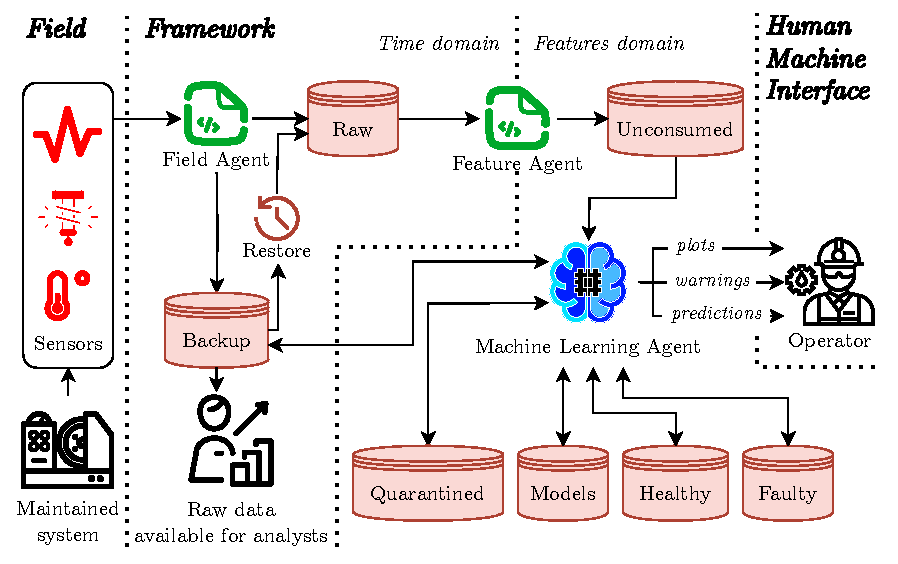
\includegraphics[width=\linewidth]{images/Framework_structure.pdf}
    \caption{The structure of the proposed framework. The Field Agent collects the time series, the Feature Agent extracts the features, and the Machine Learning Agent evaluates the health of the maintained device. The agents are connected to collections of a common database. \DIFaddbeginFL \DIFaddFL{The }
\includegraphics[height = 1em]{images/DB_icon-cropped.pdf} \DIFaddFL{icon represents a collection of a database that every agent can read and write.}\DIFaddendFL }
    \label{fig:framework_structure}
\end{figure}

The solution developed in this thesis is thought to be set up on a new device, and linked to the sensors of the most informative quantities of the system.
In the first phase of commissioning, the framework collects the data, extracts the features and stores them. When the \DIFdelbegin \DIFdel{data collected is }\DIFdelend \DIFaddbegin \DIFadd{collected data are }\DIFaddend enough to characterize all the modes of operation of the maintained system, the UML model can be trained. Finally, the framework continues collecting new \DIFdelbegin \DIFdel{data}\DIFdelend \DIFaddbegin \DIFadd{time series}\DIFaddend , extracting the features \DIFdelbegin \DIFdel{, and evaluating the new data. The framework now }\DIFdelend \DIFaddbegin \DIFadd{and evaluating these new samples. Now, the framework }\DIFaddend produces a Novelty Metric (NM) that quantifies how \DIFdelbegin \DIFdel{abnormal }\DIFdelend \DIFaddbegin \DIFadd{anomalous }\DIFaddend the new data are. 
This phase \DIFdelbegin \DIFdel{can last indefinitely }\DIFdelend \DIFaddbegin \DIFadd{lasts indefinitely (until the maintenance team performs a model update)}\DIFaddend . When the NM overshoots a certain threshold, a warning is issued to the maintenance team. 
Then, the team can \DIFdelbegin \DIFdel{then }\DIFdelend decide to perform a maintenance action or to continue monitoring the system. If \DIFdelbegin \DIFdel{they declare the }\DIFdelend \DIFaddbegin \DIFadd{the team declares the }\DIFaddend system as healthy, the framework can be retrained with the new data, to update the UML model. Otherwise, \DIFdelbegin \DIFdel{a second UML model }\DIFdelend \DIFaddbegin \DIFadd{the framework }\DIFaddend can be trained to characterize \DIFaddbegin \DIFadd{also }\DIFaddend the newly discovered fault \DIFdelbegin \DIFdel{and }\DIFdelend \DIFaddbegin \DIFadd{in order to }\DIFaddend perform Fault Detection (FD) in the future.

\subsection{Software Agents}
The proposed framework is based on software agents. Each agent is autonomous and performs a specific task. The developed agents, as shown in Fig.~\ref{fig:framework_structure}, are:
\begin{itemize}
    \item \textbf{Field Agent (FiA)}: responsible for the synchronous sampling of the data. It provides the time series records and ensures a correct sampling frequency.
    \item \textbf{Feature Agent (FA)}: extracts the features from the time series.
    \item \textbf{Machine Learning Agent (MLA)}: trains the UML algorithms and then performs ND, FD and PM. It reports the results to the user.
\end{itemize}

\subsection{Database}
All the Agents are connected to a common database. In the case of the PC implementation, MongoDB has been used. In the case of the Edge implementation, the data are stored directly in the microcontroller's memory.
Regarding the structure shown in Fig.~\ref{fig:framework_structure}, the MongoDB database is composed of seven collections. Every collection has a specific role in the framework. For example, the \emph{Quarantined, Healthy} and \emph{Faulty} collections contain the features that have been flagged as novelty, normal or faulty, respectively.

\subsection{Multiple Instances}
As shown in Fig.~\ref{fig:multiple_instances}, \DIFaddbegin \DIFadd{multiple instances of }\DIFaddend the framework can be implemented \DIFdelbegin \DIFdel{in multiple instances. This is useful }\DIFdelend to better isolate the location of the anomaly in a complex system. The larger the set of sensors that a single instance of the framework is connected to, the more difficult it is to isolate the anomaly. On the other hand, configuring a large group of sensors allows the detection of complex anomalies. 

\DIFaddbegin \DIFadd{For example, a shaft with two bearings can be monitored by two instances of the framework, one for each bearing vibration signal. Another instance can be linked to the signals of both bearings to detect more complex novelty patterns. The latter instance can exploit the case where the bearings signals are normally correlated (e.g. proportional in amplitude) to detect a novelty that is not detectable by analyzing the signals separately.   
}

\DIFaddend \begin{figure}
    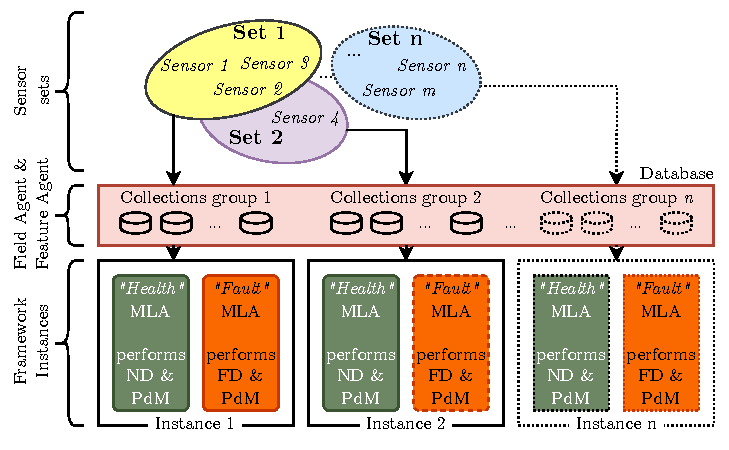
\includegraphics[width=\linewidth]{images/FrameworkInstances.pdf}
    \caption{Multiple instances implementation of the framework. Every instance is linked to a different set of sensors, to monitor different parts of the system.}
    \label{fig:multiple_instances}
\end{figure}


\subsection{Unsupervised Machine Learning Models}

The \DIFdelbegin \DIFdel{considered }\DIFdelend UML implemented in the framework are: \emph{K-means}, \emph{DBSCAN}, \emph{Gaussian Mixture Model} (GMM), \emph{Isolation Forest} (IF), \emph{Local Outlier Factor} (LOF), \emph{One-Class Support Vector Machine} ($\nu$-SVM).

K-means and DBSCAN are traditionally clustering algorithms, so a custom NM has been developed for these algorithms. \DIFaddbegin \DIFadd{For example, if K-means is used, the NM is defined as the distance of a sample from the closest centroid, normalized by the cluster radius. }\DIFaddend The other models are already commonly used for ND, so the NM has been linked to the \quoted{score} provided by the library functions.

If the UML is trained with faulty data\DIFdelbegin \DIFdel{to perform FD, the }\DIFdelend \DIFaddbegin \DIFadd{, instead of normal ones, then it performs FD. The }\DIFaddend NM measures \quoted{how not faulty} the new data are. In this case, the value is transformed into a Fault Metric (FM) with the function $\text{FM} = - \ln(\text{NM} + 1)$ to preserve the coherence \DIFaddbegin \DIFadd{(the lower the metric, the healthier the system)}\DIFaddend .  \section{FEATURE EXTRACTION}
The framework is developed to acquire time series data from an arbitrary configuration of sensors. When a time series is available, the FA extracts the features. \DIFdelbegin \DIFdel{Every }\DIFdelend \DIFaddbegin \DIFadd{Each }\DIFaddend time series is linked to a specific set of features to be extracted.

\subsection{Feature set}
The considered features are divided into two categories:
\begin{itemize}
    \item \textbf{Time domain features}: Mean, Standard deviation, Peak-to-peak value (P2P), Root Mean Square value (RMS), Skewness and Kurtosis.
    \item \textbf{Frequency domain features}: Energy of the Wavelet Packet Decomposition (WPD) coefficients, Fast Fourier Transform (FFT) coefficients. The WPD is based on the PyWavelets\footnote{\url{https://github.com/PyWavelets/pywt.git}} and Wavelib\footnote{\url{https://github.com/rafat/wavelib.git}} libraries.
\end{itemize}

The time domain features are computed in the corrected form for sampled data. In the frequency domain, the WPD is preferred in this work, because it reduces the dimensionality of the feature space. The features are standardized along the training dataset so that the mean and standard deviation are 0 and 1, respectively. This is done to ease the training of the UML algorithms.

\subsection{Scaling and selection}
\begin{figure}
    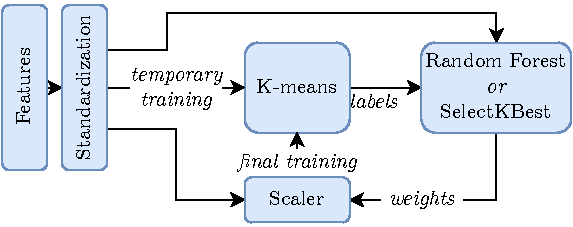
\includegraphics[width=\linewidth]{images/Feat_scaling.pdf}
    \caption{Feature scaling and selection procedure. The features are standardized and then scaled by a weight array or selected to reduce the feature space dimensionality, discarding the less informative features.}
    \label{fig:feature_scaling}
\end{figure}
Despite the standardization, during the experimental validation, it has been observed that some features are more informative than others. To reduce the impact of the less informative features, an optional feature scaling and selection step can be performed, as shown in Fig.~\ref{fig:feature_scaling}. The weights \DIFaddbegin \DIFadd{used for scaling the features }\DIFaddend can be computed by performing a Random Forest training or using the SelectKBest library method. \section{VALIDATION}
\label{sec:validation}

\subsection{On bearings vibration datasets}

The PC implementation of the framework has been thoroughly tested on a publicly available dataset collected by the Center for Intelligent Maintenance Systems (IMS).
The dataset contains time series of \DIFdelbegin \DIFdel{vibrations of bearings . It contains }\DIFdelend \DIFaddbegin \DIFadd{bearings vibrations collected during }\DIFaddend three separate \quoted{run to failure} experiences. 

\begin{figure}
    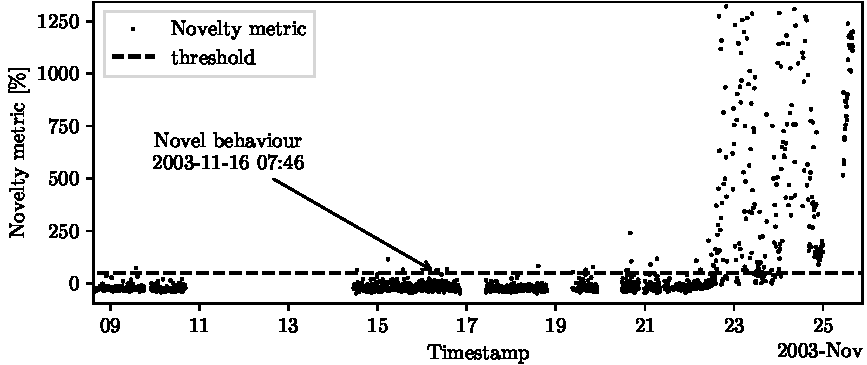
\includegraphics[width=\linewidth]{images/ND_IMS.pdf}
    \caption{Results of ND on the IMS dataset. When the Novelty Metric crosses the threshold, a warning is issued. The malfunction happens at the end of the dataset.}
    \label{fig:ND_IMS}
\end{figure}
\begin{table}
    \centering
    \caption{Comparison of the results for the test n$^\circ$1 of IMS dataset.}
    \label{tab:ims01_comparision}
    \begin{tabular}{lcrr} 
    \toprule
    \textbf{Algorithm} & \textbf{ND event} & \textbf{LT }{[}min] & \textbf{LT }{[}days] \\ 
    \hline
    K-means & 2003-11-16 07:46 & \textbf{13913} & \textbf{9.6} \\
    DBSCAN & 2003-11-22 15:06 & 4833 & 3.3\\
    GMM & 2003-11-22 03:47 & 5513 & 3.8\\
    BGMM & 2003-11-22 03:45 & 5514 & 3.8\\
    $\nu$-SVM & 2003-11-22 14:56 & 4844 &3.3\\
    IF & 2003-11-16 10:08 & 13771 & 9.6\\
    LOF & 2003-11-16 07:48 & 13912 & 9.6\\
    {P2P} without any ML & 2003-11-22 16:06 & 4774 & 3.3\\
    \bottomrule
    \end{tabular}
\end{table}
The ND capability of the framework has been tested using all the cited UML models. The Lead Time (LT) elapsed between the ND event and the actual fault is used to compare the models. The results are compared in table~\ref{tab:ims01_comparision}. The evolution of the NM, using a K-means model on a signal of the test N$^\circ$1, is shown in Fig.~\ref{fig:ND_IMS}.

\begin{figure}
    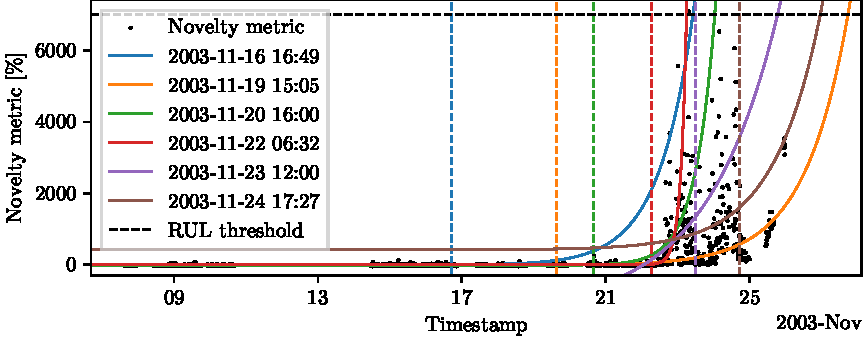
\includegraphics[width=\linewidth]{images/RUL_IMS.pdf}
    \caption{Results of Remaining Useful Life predictions on the IMS dataset. The Vertical lines indicate the time when the predictions are performed. The RUL is the time remaining before the fitted curve crosses the threshold.}
    \label{fig:RUL_IMS}
\end{figure}
To perform PM, the framework has to estimate the Remaining Useful Life (RUL) of the component. The RUL is predicted by a curve fitted to the data. The type of curve to fit is configurable\DIFdelbegin \DIFdel{, in }\DIFdelend \DIFaddbegin \DIFadd{. In }\DIFaddend this work $y = a \cdot e^{b \cdot x} + c$ has been used. The results of the RUL predictions are shown in Fig.~\ref{fig:RUL_IMS}.

\begin{figure}
    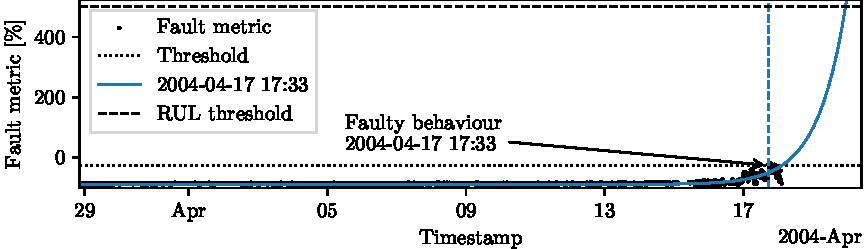
\includegraphics[width=\linewidth]{images/FD_IMS.pdf}
    \caption{Results of FD on the IMS dataset. The malfunction is detected when the Fault Metric crosses the threshold. The RUL is the time remaining before the fitted curve crosses the threshold.}
    \label{fig:FD_IMS}
\end{figure}
Since the second and third tests of the IMS dataset share the same type of fault, the framework has been trained to perform FD with the faulty data of the second test and then \DIFaddbegin \DIFadd{it has been }\DIFaddend evaluated on the third \DIFaddbegin \DIFadd{test}\DIFaddend . Analogously to the ND, \DIFdelbegin \DIFdel{after }\DIFdelend \DIFaddbegin \DIFadd{when }\DIFaddend the FM crosses a certain threshold, a warning is issued and RUL predictions are performed. The results of the FD are shown in Fig.~\ref{fig:FD_IMS}.

\subsection{Laboratory tests}

\begin{figure}
    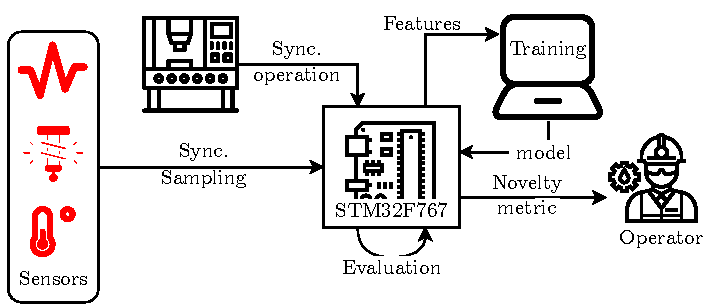
\includegraphics[width=\linewidth]{images/EmbeddedStructure.pdf}
    \caption{Structure of the Edge implementation. The microcontroller autonomously evaluates the status of the maintained system. Only during the training phase, the PC implementation computes the model for the Edge.}
    \label{fig:embedded}
\end{figure}

K-means, IF and LOF are the three models that performed the best on the dataset. \DIFdelbegin \DIFdel{K-means performed equally or only slightly better than IF and LOF. }\DIFdelend Notably, the K-means model has advantages such as minimal parameter storage requirements and low computational costs for calculating the NM. For these reasons, the K-means model has been chosen for the Edge implementation.

In the first phase, the framework gathers the data and extracts the features. The UML model is trained on a PC and then included in the Edge. After, the microcontroller autonomously evaluates the status of the maintained system. The structure of the Edge implementation is shown in Fig.~\ref{fig:embedded}. 

\begin{figure}
    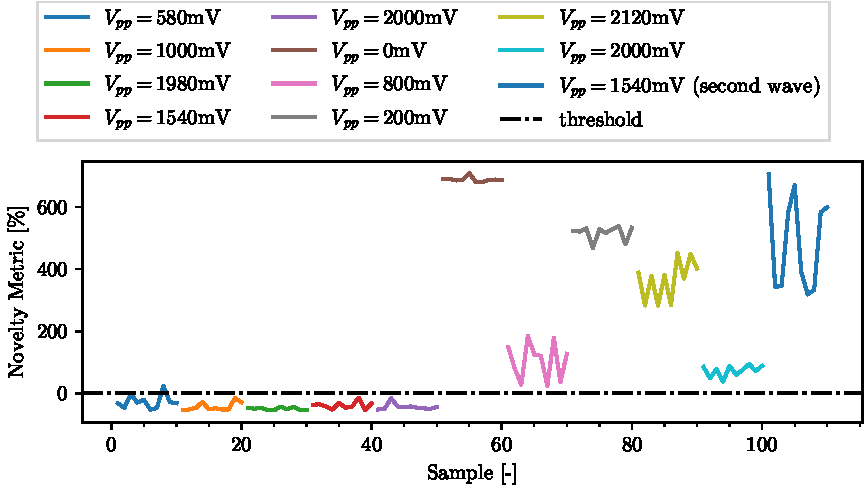
\includegraphics[width=\linewidth]{images/Test02_LOF.pdf}
    \caption{Results of \DIFaddbeginFL \DIFaddFL{a }\DIFaddendFL laboratory test on the shaker. The first five lines are evaluations of known vibrations, correctly flagged as normal samples. The remaining lines are the successful detections of the novelty of new vibrations.}
    \label{fig:shaker}
\end{figure}

Extensive tests have been performed on a laboratory shaker, simulating the vibrations generated by a generic mechanical system. The tests have been carried out to evaluate the sensitivity to variations in both amplitude and frequency content. The results of \DIFdelbegin \DIFdel{the ND }\DIFdelend \DIFaddbegin \DIFadd{a ND test }\DIFaddend are shown in Fig.~\ref{fig:shaker}.

A second series of tests has been performed mounting the accelerometer on a linear actuator. The axis of the accelerometer has been aligned with the direction of the movement of the actuator \DIFdelbegin \DIFdel{, to sense more the acceleration actuated }\DIFdelend \DIFaddbegin \DIFadd{to sense the actuated acceleration, }\DIFaddend rather than the vibrations. A set of predefined movement profiles has been used for training, while another set for testing. This series of tests exploited a high number of non-significant features. This is because the WPD gave high resolution \DIFdelbegin \DIFdel{on }\DIFdelend \DIFaddbegin \DIFadd{over }\DIFaddend a wide range of frequency content, but the actuator excited only a few, and very low, frequencies. The remaining features were almost all noise, and the standardization procedure had the side effect of amplifying them to the same level as the significant ones. An effort has been made to fine-tune the model to reduce the impact of the noise (see Fig.~\ref{fig:linear}, models 1 to 4). The best result, however, has been obtained by removing the less informative features and using a reduced feature space. The benefit of this approach is evident in Fig.~\ref{fig:linear}.


\begin{figure}
    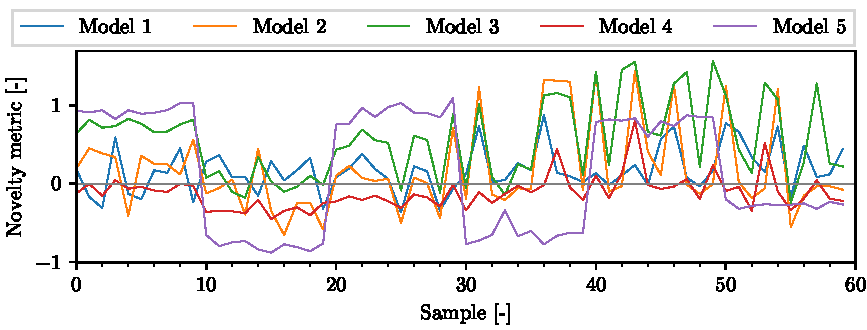
\includegraphics[width=\linewidth]{images/linear.pdf}
    \caption{Results of laboratory test on linear actuator acceleration profiles. The dimensionality of the feature space has been reduced to train Model~5, which performs a clear and sharp detection of the alternating pattern between known and unknown movement profiles.}
    \label{fig:linear}
\end{figure} \section{CONCLUSION AND FUTURE WORK}

The proposed solution has been proven effective in performing Novelty Detection in both public datasets and laboratory tests. The flexibility of the framework allows it to be easily adapted to different systems. 

Some laboratory tests on the Edge implementation have shown that the standardization of the features is not always enough to make the clusters in the feature space meaningful. When this happened, \DIFdelbegin \DIFdel{in the PC implementation, }\DIFdelend Isolation Forest and Local Outlier Factor \DIFdelbegin \DIFdel{Models}\DIFdelend \DIFaddbegin \DIFadd{models were tested in the PC implementation and}\DIFaddend , being not cluster-based, \DIFdelbegin \DIFdel{were tested and resulted as }\DIFdelend \DIFaddbegin \DIFadd{proved to be }\DIFaddend more effective. As future work, the deployment of these models also in the Edge implementation would improve the performance of the \DIFaddbegin \DIFadd{Edge }\DIFaddend framework in some specific applications. 
\end{document}
